\subsection{HOPR incentivization mechanism}
HOPR incentivizes nodes in order to achieve correct transformation and delivery of mixnet packets. 
This is accomplished using a mechanism called “Proof-Of-Relay” with the following second-layer solutions which are both cost effective and privacy preserving.

\subsubsection{Probabilistic payments within payment channels}
In payment channels, two parties A and B lock some funds within a smart contract, make multiple transactions off-chain and only commit the aggregation on-chain. 
This implies that the last HOPR acknowledgement contains all previous incentives plus the incentive for the most recent interaction 
   $$value(ACK_n) =\sum_{i=1}^nfee(packet_i)$$
If B received $ACK_n$ before sending $packet_{n-1}$, it has no incentive to process $packet_{n-1}$ rather than $packet_{n-2}$. 

\subsubsection*{Probabilistic payments}  
The payouts use a concept called “tickets”. In this scheme, there is a known selection rate $s$ (assuming $s=1000$).
A ticket can be a win or a loss with $\frac{1}{1000}$ probability which means nodes are incentivized to continue relaying packets as they don’t know which ticket is a win. 
\\~\\HOPR uses a custom-made second-layer solution. It is inspired by payment channels and probabilistic payments where incentives can be claimed independently: 
$$value ( ACK_i )=value ( ACK_j ) \quad for \quad i,j\in \{1,n\}$$
Hence, there is no added value in pretending packet loss or intentionally changing the order in which packets are processed. 
\subsubsection*{Privacy challenges}
The incentives break the unlinkability guarantees inherited from the SPHINX packet format as they reveal the identity of the packet origin who transfers those incentives in the channel using their signature. 
\\To solve this problem, HOPR forward incentives next to the packet.
\begin{figure}[H]
    \centering
    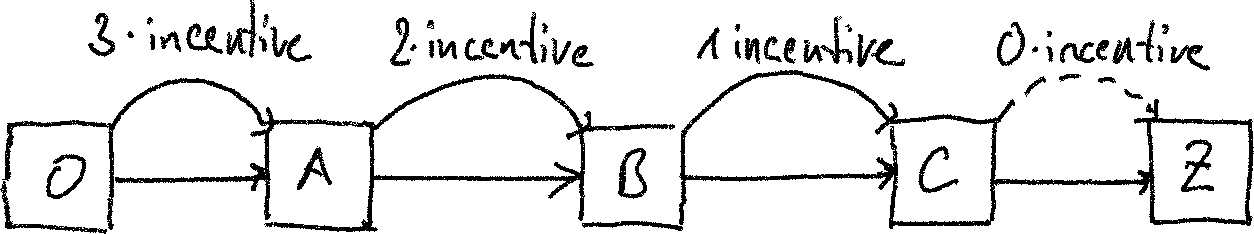
\includegraphics[width=10cm,height=10cm,keepaspectratio]{../whitepaper/images/token_cashflow.png}
    \caption{Incentive flow}
    \label{fig:Incentive flow}
    \end{figure}

    \hspace{-5mm}This however leaks the relayer’s position within the selected path since the value of the ticket is set according to the current relay fee and the number of intermediate hops, 
more precisely $$amount:=\frac{(hops -1)* relayFee}{winProb}$$
This leakage is considered to have a low severity but further research will be conducted on the subject.
\subsubsection{Proof Of Relay}

HOPR incentivizes packet transformation and delivery using a mechanism called “Proof-Of-Relay”. 
This mechanism makes sure nodes relay services are verifiable.
\paragraph{Construction} 
\begin{itemize}
    \item Every packet is sent together with a ticket. 
    \item Each ticket contains a challenge.
    \item The validity of a ticket can only be checked on reception of the packet but the on-chain logic enforces a solution to the challenge stated in the ticket.
\end{itemize}
Since “Proof-Of-Relay” is used to make the relay services of nodes verifiable, it is the duty of each node to check that given challenges are derivable from the given and the expected information. 
Packets with inappropriate challenges should be dropped as they might not lead to winning tickets.
Therefore, the sender of the packet also provides a hint of the expected value that a node is supposed to get from the next downstream node (as explained in the ticket section). 



\subsubsection{The Importance of Stake}
In order to incentivize reliable connections, we require payment channels to be staked. We also assume stake is correlated with availability and thus with reputation. Therefore, weighing by stake the selection of which mix nodes to include in the channel graph results in a mixnet populated by nodes that have the reputation of offering a high quality of service.
 Staking is also a countermeasure for sybil attacks, as creating many node identities becomes expensive. 








